\documentclass{article}
\usepackage{amsmath,amsthm,amssymb}
\usepackage {mathtext}
\usepackage{amsfonts} 
\usepackage[T1,T2A]{fontenc}
\usepackage[utf8]{inputenc}
\usepackage [english, russian] {babel}
\usepackage[babel=true]{microtype}
\usepackage{caption}
\usepackage{subcaption}
\captionsetup[table]{position=t,justification=raggedleft,slc=off}
\setlength{\abovecaptionskip}{0pt}
\usepackage {geometry}
\usepackage{graphicx}
\geometry{margin=1in}
\title{Лабораторная работа №1.2.1. \\ Определение скорости полёта пули при помощи баллистического маятника}
\author{Павел Рудачихин \\ Б04-507}
\date{30.10.2025}
\begin {document}
\maketitle{}
\section* {Аннотация} 

\hspace{4mm} В работе определяется скорость полёта пули. Исследуются погрешности проводимых измерений.

\textbf{Цель работы:} определить скорость полёта пули, применяя законы сохранения и используя баллистические маятники.

\textbf{В работе используются:} духовое ружьё на штативе, осветитель, оптическая система для измерения отклонения маятника, измерительная линейка, рулетка, пули и весы, баллистические маятники.

\textbf{Методы:} 1) измерение изменения положения маятника с помощью линейки-шкалы; 2) измерение геометрических размеров с помощью линейки; 3) измерение массы тел с помощью весов; 4) измерение расстояния с помощью рулетки.

\section* {Теоретические сведения}

\hspace{4mm} Непосредственно измерить скорость пули сложно без дорогостоящей аппаратуры для регистрации быстропеременных процессов. Поэтому в работе скорость пули определяется по импульсу, передаваемому ею баллистическому маятнику при неупругом соударении. \textit{Баллистический маятник} - маятник, колебания которого вызываются кратковременным начальным импульсом (толчком), т.е. время соударения гораздо меньше периода колебаний. 

Длительность соударения пули и маятника можно оценить по глубине проникновения пули, полагая силу сопротивления постоянной: при скорости 200 м/с глубина $\approx 1 $ см, значит время удара $\approx 10^{-4}$ с.

При кратковременном ударе даже в присутствии внешних сил можно применить \textbf{закон сохранения импульса} (далее - ЗСИ) для системы "пуля - маятник".

При малых затуханиях колебаний можно применить \textbf{закон сохранения механической энергии} (далее - ЗСЭ), чтобы по максимальному отклонению маятника определить его начальную скорость. В работе малость затухания определяется уменьшением амплитуды менее, чем наполовину за 10 колебаний.

\section* {Методика измерений}

\subsection* {Поступательный баллистический маятник}

\hspace{4mm} Маятник, изображённый на рис. 1 и используемый в первой части работы, представляет собой тяжёлый цилиндр, подвешенный на четырёх нитях одинаковой длины. При колебаниях центр масс цилиндра перемещается по дуге окружности радиуса $L$ (см. рис. 2).

\begin{figure}[h!]
	\centering
	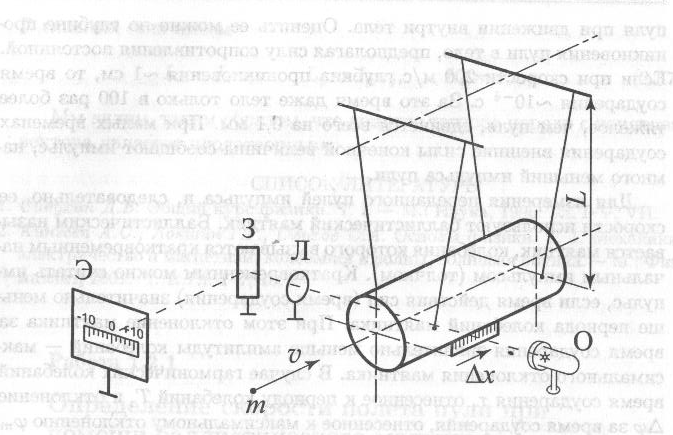
\includegraphics[width=0.6\linewidth]{1}
	\caption{Схема первой установки: Э - экран, З - зеркало, Л - линза, О - осветитель.}
	\label{fig:1}
\end{figure}

\begin{figure}[h!]
	\centering
	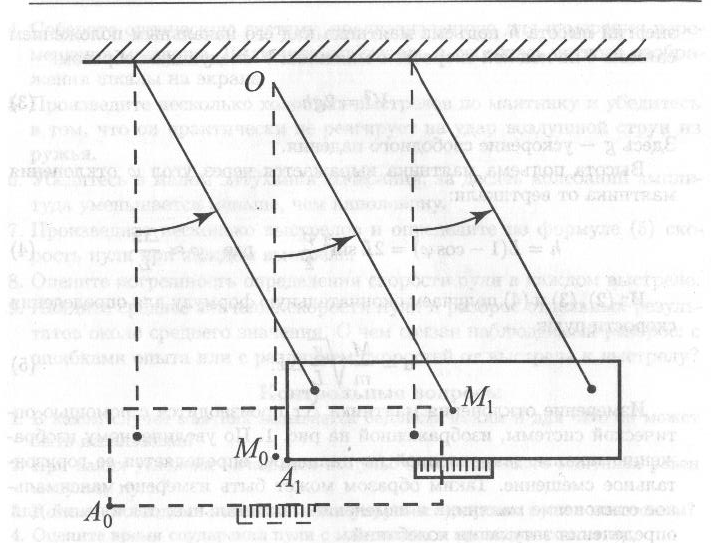
\includegraphics[width=0.6\linewidth]{2}
	\caption{Схема первой установки: $M_0$ - начальное положение центра масс, $M_1$ - конечное положение центра масс. OM = L.}
	\label{fig:2}
\end{figure}


Применяя полученные ранее приближения и пренебрегая массой пули по сравнению с массой цилиндра, получим по ЗСИ:

\begin{equation}
	u = \frac{M}{m}V,
\end{equation}

где $u$ - скорость пули до удара, $M$ - масса маятника, $m$ - масса пули, $V$ - начальная скорость цилиндра после удара.

По ЗСЭ начальная кинетическая энергия маятника переходит в потенциальную энергию в поле тяжести. Пусть максимальная высота подъёма $h$, тогда

\begin{equation}
	V^2 = 2 g h,
\end{equation}

где g - ускорение свободного падения.

Пусть $\varphi$ - угол отклонения маятника от вертикали. При малых отклонениях по горизонтали $\Delta x$:  $\varphi \approx \Delta x / L$. Связь высота подъёма и горизонтального смещения из геометрических соображений:

\begin{equation}
	h = L(1 - \cos \varphi) = 2L\sin^{2} \frac{\varphi}{2} \approx 2 L (\frac{\Delta x}{2L})^{2} = \frac{\Delta x^{2}}{2L}
\end{equation}

Подставив в формулу (2) имеем:

\begin{equation}
	V = \sqrt{2gh} = \sqrt{2g\frac{\Delta x^{2}}{2L}} = \Delta x \sqrt{\frac{g}{L}}
\end{equation}

Подставив в формулу (1), получаем окончательное выражение для определения скорости пули:

\begin{equation}
	u = \frac{M}{m} \sqrt{\frac{g}{L}} \Delta x 
\end{equation}

\subsection* {Крутильный баллистический маятник}

\hspace{4mm} Маятник, изображённый на рис. 3 и используемый во второй части работы, представляет собой вертикальную ось с горизонтальным стержнем, на котором симметрично оси закреплены мишени и грузы. 

\begin{figure}[h!]
	\centering
	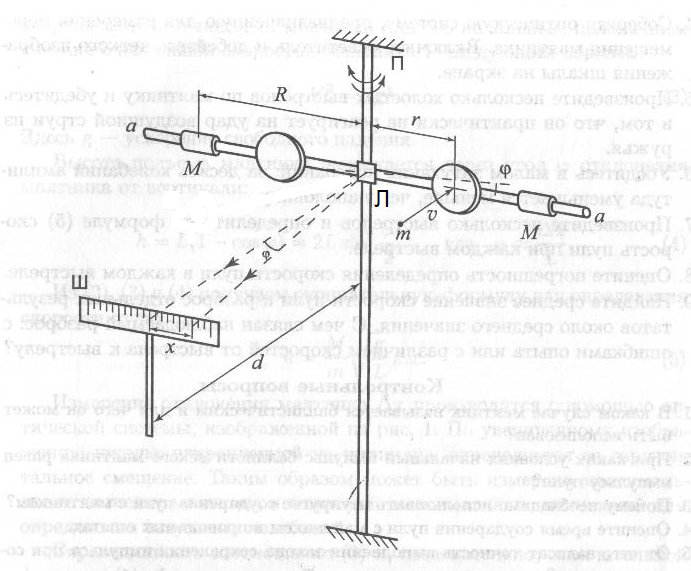
\includegraphics[width=0.7\linewidth]{3}
	\caption{Схема второй установки: П - проволока, М - груз, аа - стержень, перпендикулярный проволоке, Ш - шкала, Л - лазерный указатель.}
	\label{fig:3}
\end{figure}



Используем \textbf{закон сохранения момента импульса} (далее - ЗСМИ). Его применимость обусловлена малым временем удара по сравнению с периодом колебаний маятника (аналогично ЗСИ). Имеем:

\begin{equation}
	mur = I \Omega,
\end{equation}

где $r$ - расстояние от линии полёта пули до оси, $I$ - момент инерции маятника, $\Omega$ - угловая скорость маятника после удара.

Пренебрегая потерями на трение, запишем ЗСЭ:

\begin{equation}
	k\frac{\varphi^2}{2} = I\frac{\Omega^2}{2}
\end{equation}

Из (6) и (7) получаем :

\begin{equation}
	u = \varphi \frac{\sqrt{kI}}{mr}
\end{equation}

Аналогично первой части:

\begin{equation}
	\varphi \approx \frac{\Delta x}{d},
\end{equation}

где $d$ - расстояние от шкалы до оси.

$kI$ можно определить, измерив период колебаний маятника с грузами массы $m_1, \ m_2$ и без них, используя аддитивность момента инерции:

\begin{equation}
	T_1 = 2 \pi \sqrt{\frac{I}{k}}; \ \ \ T_2 = 2 \pi \sqrt{\frac{I - (m_1 + m_2)R^2}{k}},
\end{equation}

где $R$ - расстояние от центров масс грузов до оси. Следовательно,

\begin{equation}
	\sqrt{kI} = \dfrac{2 \pi (m_1 + m_2) R^2 T_1}{T_1^2 - T_2^2}
\end{equation}

Окончательная формула для скорости пули в этом опыте:

\begin{equation}
	u = \frac{\Delta x}{m}\dfrac{2 \pi (m_1 + m_2) R^2 T_1}{r d (T_1^2 - T_2^2)}
\end{equation}

Удобно далее обозначить правую дробь как постоянную $\lambda$. 

\section*{Используемое оборудование}

\hspace{4mm} В данной работе для измерения массы использованы цифровые \textbf{весы}. Погрешность измерения массы определена по инструкции прибора: $\Delta_{\text{m}} = \pm 5$ мг

Погрешность \textbf{первой линейки-шкалы} составляет $\Delta_{\text{l1}} = \pm 0,25$ мм 

Погрешность \textbf{второй линейки-шкалы} составляет $\Delta_{\text{l2}} = \pm 0,5$ мм 

Погрешность \textbf{рулетки} определена ценой деления: $\Delta_{\text{L}} = \pm 1$ мм

Погрешность цифрового \textbf{секундомера} определена как три в последнем разряде: $\Delta_{\text{t}} = \pm 0,03$ c


\section*{Результаты измерений}

\subsection*{Параметры установки}

\hspace{4mm} Параметры установок приведены в таблицах 1 и 2.  

\begin{table}[h!]
	\centering
	\captionbox{Параметры первого маятника}{
		\begin{tabular}{|c|c|}
			\hline
			Параметр  & Значение  \\
			\hline
			Масса маятника, $M$ & $(295 \pm 5)$ г \\
			\hline
			Высота подвеса, $L$  & $(222 \pm 1)$ мм  \\
			\hline
			
	\end{tabular}}

\end{table}

\begin{table}[h!]
	\centering
	\captionbox{Параметры крутильного маятника}{
		\begin{tabular}{|c|c|}
			\hline
			Параметр  & Значение  \\
			\hline
			Расстояние от шкалы до оси, $d$ & $(140 \pm 1)$ см \\
			\hline
			Расстояние от центра мишени до оси, $r$  & $(205 \pm 1)$ мм  \\
			\hline
			Расстояние от центра масс груза до оси, $R$  & $(340 \pm 1)$ мм  \\
			\hline
			Масса грузов, $m_1, m_2$  & $(733,2 \pm 0,5)$ г, $(735,5 \pm 0,5)$ г  \\
			\hline
			
	\end{tabular}}
\end{table}

Результаты измерений масс пуль представлены в таблице 3.

\begin{table}[h!]
	\centering
	\captionbox{Измерение масс пуль}{
		\begin{tabular}{|r|r|r|r|r|r|r|r|r|r|r|}
			\hline
			№ & 1     & 2     & 3     & 4     & 5     & 6     & 7     & 8 & 9  & 10 \\
			\hline
			$m$, мг & 506     & 512     & 518     & 501     & 505     & 499    & 506     & 507 & 502 & 499 \\
			\hline
	\end{tabular}}
\end{table}

Результаты измерения времени десяти колебаний крутильного маятника с грузами и без представлены в таблице 4.

\begin{table}[h!]
	\centering
	\captionbox{Время 10 колебаний, с}{
		\begin{tabular}{|c|c|}
			\hline
			С грузами  & Без грузов  \\
			\hline
			65,47 & 47,56 \\
			\hline
			65,57 & 47,38 \\
			\hline
			65,30 & 47,43 \\
			\hline
			
			
	\end{tabular}}

	
\end{table}

Смещения маятников указаны в таблице 5.

\begin{table}[h!]
	\centering
	\captionbox{Смещение маятников (лазерных меток)}{
		\begin{tabular}{|c|c||c|c|}
			\hline
			№ & $\Delta x$, мм & № & $\Delta x$, cм  \\
			\hline
			1 & 9,00 & 6 & 4,75 \\
			\hline
			2 & 9,00 & 7 & 4,80 \\
			\hline
			3 & 10,00 & 8 & 4,35 \\
			\hline
			4 & 10,50 & 9 & 4,00 \\
			\hline
			5 & 9,75 & 10 & 3,80 \\
			\hline
			
			
	\end{tabular}}
\end{table}

\section*{Обработка результатов}

Для определения погрешности измерения суммарной массы грузов использована формула:

\begin{equation}
	\sigma_{m_1+m_2}^2 = \sigma_{m_1}^2 + \sigma_{m_2}^2
\end{equation}

Относительная погрешность скорости в первом опыте определена следующим образом:

\begin{equation}
	\varepsilon_{u}^2 = \varepsilon_{M}^2 + \varepsilon_{m}^2 + (-0,5)^{2}\varepsilon_{L}^2 + \varepsilon_{\Delta x}^2
\end{equation}

Относительная погрешность константы определена аналогично:

\begin{equation}
	\varepsilon_{\lambda}^2 = \varepsilon_{m_1+m_2}^2 + 4\varepsilon_{R}^2 + \varepsilon_{T_1}^2 + \varepsilon_{r}^2 + \varepsilon_{d}^2 + \varepsilon_{T_1^2 - T_2^2}^2
\end{equation}

Последнее слагаемое вычислено так:

\begin{equation}
	\varepsilon_{T^2}^2 = 4 \varepsilon_{T}^2; \  \varepsilon_{T^2} = 2 \varepsilon_{T}; \
	\sigma_{T^2} = T^2 \varepsilon_{T^2}; \
	\sigma_{T_1^2 - T_2^2}^2 = \sigma_{T_1^2}^2 + \sigma_{T_2^2}^2; \
	\varepsilon_{T_1^2 - T_2^2} = \frac{\sigma_{T_1^2 - T_2^2}}{T_1^2 - T_2^2}.
\end{equation}

Относительная погрешность скорости во втором опыте определена следующим образом:

\begin{equation}
	\varepsilon_{u}^2 = \varepsilon_{\Delta x}^2 + \varepsilon_{m}^2 + \varepsilon_{\lambda}^2 
\end{equation}

При определении периода колебаний во втором опыте посчитано среднее значение времени и случайная погрешность, равная среднеквадратичному отклонению. Полная погрешность определена по случайной и систематической аналогично (13).
 
\begin{equation}
	T_1 = (6,545 \pm 0,011) \ с; \ T_2 = (4,746 \pm 0,008) \ с
\end{equation}

Вычислена константа:

\begin{equation}
	\lambda = (1,34 \pm 0,02) \ кг/с
\end{equation}

Полученные значения скоростей пуль представлены в таблице 6. Систематическая погрешность в первом опыте составила 2 м/с, во втором - 3 м/с. Случайная погрешность в первом опыте равна 8 м/с, во втором - 10 м/с. Полная погрешность составила 8 м/с в первом опыте и 10 м/с во втором.

\begin{table}[h!]
	\centering
	\captionbox{Результаты измерений скорости пули}{
		\begin{tabular}{|c|c||c|c|}
			\hline
			№ & $u$, м/с & № & $u$, м/с  \\
			\hline
			1 & 110 & 6 & 128 \\
			\hline
			2 & 109 & 7 & 127 \\
			\hline
			3 & 120 & 8 & 115 \\
			\hline
			4 & 130 & 9 & 107 \\
			\hline
			5 & 120 & 10 & 102 \\
			\hline
		\end{tabular}}
\end{table}

Получены следующие средние значения скоростей в первом и втором опыте соответственно:

\begin{equation}
	\boxed{ u_1 = (116 \pm 8) \ м/с \ \ \ \ u_2 = (118 \pm 10) \ м/с}
\end{equation}

Все вычисления произведены с использованием программы, написанной специально для этих целей на языке программирования Python. Исходный код программы содержится в электронном приложении к работе.




 

\section*{Анализ результатов}

\hspace{4mm} Согласно справочным данным, скорость вылета пули из духового ружья меняется в широких пределах и обычно составляет 150 - 200 м/с \footnote[1]{А.Д. Гладун и др. Лабораторный практикум по общей физике - М.: МФТИ, 2012.}. Отметим, что используемое в первом опыте ружьё относительно слабое, а во втором опыте использован пистолет. Поэтому полученный результат является ожидаемым. 

Наибольший вклад в итоговую систематическую погрешность вносит измерение угла. Действительно, при смещении на 9,75 мм и инструментальной погрешности в 0,25 мм относительная погрешность измерения смещения превышает 2,5\%. Кроме того, высока случайная погрешность измерения времени колебаний маятника. Это может быть связано со скоростью реакции наблюдателя с секундомером. Избежать этой ошибки можно, используя датчик (например, на оптопаре) или видеосъёмку с высокой частотой кадров.

В полную погрешность результата наибольший вклад вносит случайная погрешность. Скорее всего, это обусловлено конструкцией ружья и пистолета. Заметим, что скорость пули во втором опыте строго убывает. Значит, уменьшается сила, разгоняющая пулю. Это указывает на то, что источником сжатого воздуха в пистолете является баллон, давление в котором с каждым выстрелом уменьшается. В первом опыте нет закономерности в значениях скоростей. Возможно, в ружье использован пружинно-поршневой механизм. Одним из его недостатков является, как раз, нестабильная скорость вылета пули. Это обусловлено вибрациями ружья в момент выстрела из-за удара поршня и износом пружины.  


\section*{Заключение}
\hspace{4mm} Цель работы достигнута: измерена скорость вылета пули из духового ружья. Вычислены погрешности проведённых измерений. Определены возможные источники ошибок.

\end {document}